\documentclass{cshonours}
\bibliographystyle{acm}

\usepackage{graphics}  %optional
\usepackage{algorithm,algorithmicx,algpseudocode}
\usepackage[scientific-notation=true]{siunitx}

\title{RNA Folding: Beyond the Thermodynamic Hypothesis}
\author{Max Ward (20748588)}

\keywords{Ribonucleic acid, secondary structure, prediction}
\categories{J.3 Biology and genetics}

\begin{document}
\maketitle

\begin{abstract}
Algorithmic prediction of Ribonucleic Acid (RNA) secondary structure has been actively researched since the 1970s. RNA is a biologically active molecule with many poorly understood functions. Quick and accurate prediction of RNA structure is therefore essential for further elucidation of its role. The Thermodynamic Hypothesis, which is the fundamental dogma underlying protein folding algorithms, has been applied successfully to the RNA folding problem. Unfortunately, this success is only partial; RNA folding algorithms are currently not able to reliably predict correct structures. These algorithms typically globally optimize some scoring function, usually thermodynamic stability. This is in keeping with the Thermodynamic Hypothesis. In this investigation I hypothesize that local interactions are stronger than global interactions during RNA structure formation. Locally optimal windows were merged into complete secondary structures. These were more accurate than corresponding globally optimal structure, using the same model of RNA folding. I argue that this constitutes strong support for my hypothesis. In addition, a new algorithm called `$ab$-splat', which is based on the computation of locally optimal windows, is introduced. This algorithm, while very naive, has comparable prediction accuracy to the RNAfold algorithm on which it is based (part of the popular Vienna RNA Suite). Additionally, it runs an order of magnitude faster, and uses less memory.
\end{abstract}

\begin{acknowledgements}
Going to need something here too.
This class is designed to produce reports that look
the same as those produced by the older {\tt cshonours.sty} style for
\LaTeX 2.09, which was modified by Nick Spadaccini from a style
provided by Ken Wessen.
\end{acknowledgements}

\tableofcontents
\listoftables  %optional
\listoffigures  %optional



\chapter{Introduction}
The algorithmic prediction of Ribonucleic Acid (RNA) secondary structure is practically and theoretically important. The subject has been actively researched since the early 1970s. Despite this, current techniques are often unreliable, and are unable to accurately predict the structures of some RNAs. This is especially true for algorithms that make predictions without any form of consensus matching against known RNAs. Unfortunately these are the most generally useful algorithms as they can predict RNA structure given only the RNA sequence itself. This may be because they attempt to globally optimize some scoring function; typically the scoring system reflects thermodynamic stability. The core hypothesis of this investigation is that local interactions can be stronger than global interactions during RNA structure formation. Additionally, such interactions can improve the prediction accuracy using our current best models of RNA. If these hypotheses are supported, it follows that improvements in algorithmic prediction of RNA secondary structure can be achieved. However, to understand the importance of RNA we must first understand the better know Deoxyribonucleic Acid (DNA).


\chapter{Relevant Literature}


\section{DNA and RNA}
DNA is the basic genetic building block upon which the classification of genetic material into genes and chromosomes is based. The role of DNA as the hereditary unit of genetics was determined in the 1940s \cite{albertsessential}. Soon thereafter, Watson \& Crick \cite{watson1953molecular} published a highly acclaimed paper describing the fundamental chemical structure of DNA. In it, they outlined a double helix formation which has since become as iconic as it is canonical (see Figure \ref{dna}). Each strand of the helix Watson \& Crick discovered is essentially a chain of `nucleotides'. Each nucleotide is made of a sugar-phosphate backbone attached to a single `base'. The bases of corresponding strands form hydrogen bonds which hold the double helix together. The most astonishing and important of their findings was that these bases bond in a reciprocal fashion. They described four bases: Adenine (A), which always bonds to Thymine (T), and Guanine (G), which always bonds to Cytosine (C).

\begin{figure}
\begin{center}
\scalebox{0.23}{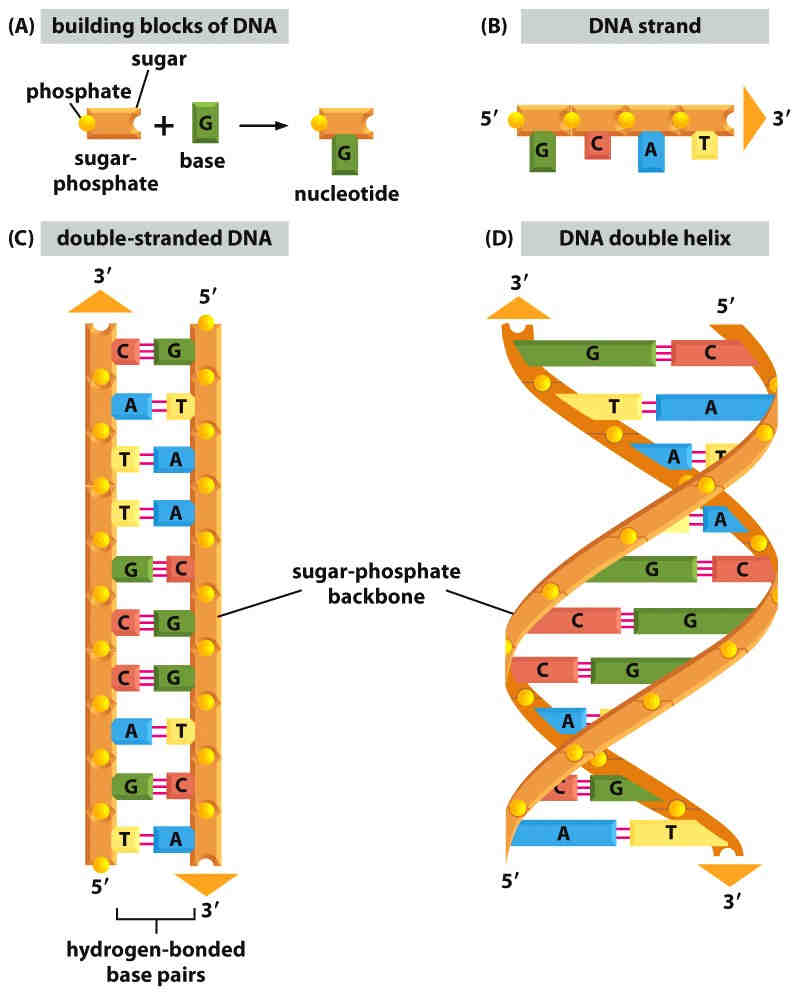
\includegraphics{dna}}
\end{center}
\caption{The structure and composition of DNA. Diagram taken from \emph{Essential Cell Biology} \cite{albertsessential}.}
\label{dna}
\end{figure}

The reciprocal bonding relationships between bases is what allows replication to occur; a copy of DNA can be made by allowing the correct bases to bond to one of the strands making up its helix. This gives a model for inheritance and cellular replication. However, there remains the question of how DNA can actually code for protein. Proteins are made up amino acids bonded in a specific sequence \cite{albertsessential}. The DNA must therefore code for amino acids. This code, which can be thought of as the `digital' representation for the `analogue' protein used by our cells, needs to be carried to ribosomes which translate it into protein \cite{albertsessential}. This is a task carried out by RNAs. RNA is very much like DNA in that it can bond reciprocally to another strand with matching bases. The main difference is that it is single stranded in structure, and has Uracil (U) in place of Thymine \cite{albertsessential}. It is important to note that in RNA molecules G and U pairings are also possible. RNA bonds to DNA and, in a sense, reads it. This results in the production of a copy of the DNAs genetic payload. This `downloaded' information is then carried away to be translated into protein \cite{albertsessential}. An example of this is depicted in Figure \ref{transcription}, in which we see a Messenger RNA molecule bonding to and thus making a copy of a section of DNA. As depicted in Figure \ref{transcription}, the 3' end of a DNA or RNA molecule is the end onto which new nucleotides are added. The 5' end is chemically stable, and nucleotides are not usually appended to it \cite{albertsessential}.

\begin{figure}
\begin{center}
\scalebox{0.23}{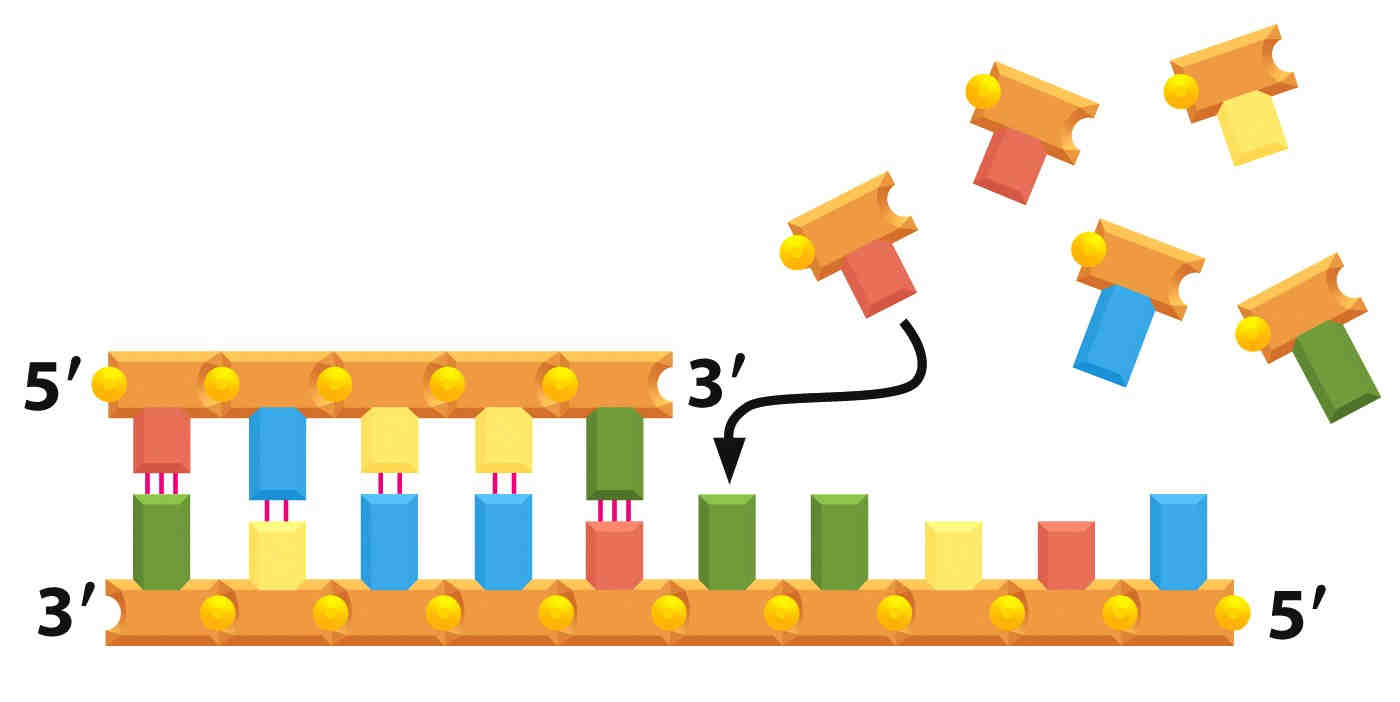
\includegraphics{transcription}}
\end{center}
\caption{RNA transcription. Diagram taken from \emph{Essential Cell Biology} \cite{albertsessential}.}
\label{transcription}
\end{figure}



For many years the conventional wisdom was that DNA contained genes which coded for functional proteins used by the cell \cite{albertsessential}. Though this is undoubtedly true, there was a problem: much of the human genome, and the genomes of other species, contains DNA which does not appear to code for anything \cite{beaton1999eukaryotic}. Many theories have been put forward to explain this. It was argued that this `junk' DNA is the perennial build-up of mutation, and that natural selection simply cannot act with strong enough selective force to cull this free-loading DNA \cite{beaton1999eukaryotic}. Surprisingly, much of this non-coding DNA is transcribed into RNA, despite having no apparent function \cite{leung2013coral}. 

As it turns out, RNA is more than a simple messenger for encoded proteins. Recent research has found myriad important functions for RNA. For example, RNA can act as a catalyst for mRNA splicing and peptide bond formation, and can also alter the regulation of genes \cite{xu2012statistical}. It seems that much of our genome contains templates for non-coding RNAs (ncRNAs). These RNAs perform essential cellular functions without actually being translated into protein at any point in their life-cycle \cite{leung2013coral}. Because of its inherently single stranded nature, RNA forms bonds with itself, folding into secondary and tertiary structures \cite{conn1998rna}.


It is axiomatic that chemical structure is tantamount to biological function; RNA is no exception. For this reason there has and continues to be an intense interest in predicting the secondary and tertiary structure of RNA molecules. This is in part because it will elucidate the underlying principles of RNA structure formation and function \cite{conn1998rna}, but also because it will allow the detection and classification of unknown RNAs, enable prediction of novel RNA function, and assist the design of new RNA based drugs \cite{condon2003problems}. In fact, RNA is an extremely versatile molecule, and as such is attractive from both an engineering, and computational point of view. Small combinatorial computational problems have been solved by representing the solution set using RNAs. Furthermore, a theory of computation has been put forward using self assembling RNA molecules \cite{condon2003problems}. As if to comment on the upheaval of a protein-centric view of biology in recent years, researchers have found that RNA is capable of supporting all the processes required for life without needing proteins \cite{condon2003problems}. The secondary structure of RNA is also highly conserved during evolution, indicating its importance \cite{hofacker2008rna}. 

Secondary and tertiary structures can be treated hierarchically. As a result, it is possible to predict the secondary structure of an RNA without understanding the tertiary structure. The tertiary structure in turn builds upon the secondary structure \cite{tinoco1999rna}. This paper will focus on secondary structure prediction.

It holds to reason that an algorithm for RNA secondary structure prediction can never be realised if we do not understand how these structures form, or their general morphology. For this reason it is important to understand how true RNA secondary structures can be determined, and the limitations of these techniques. DNA and RNA molecules can be analysed using X-ray crystallographic methods. These types of approaches work because the wavelengths of some X-rays are the same as the dimensions of DNA and RNA inter-atomic bonds. The diffraction of X-ray light by these molecules can thus be observed, and their structures can subsequently be inferred by analysis of the resulting data. Nuclear Magnetic Resonance (NMR) is another technique which can be applied to the analysis of DNA or RNA. It relies on the spin of atoms when in a magnetic field. These spin signals can be used to determine the atomic composition and topology of a molecule. This has the advantage of not requiring the molecule under observation to be crystallized before analysis. Arguably NMR gives a better in vivo view of RNAs and DNAs, which are fundamentally flexible structures. NMR also has some disadvantages; for instance, it is less accurate than X-ray crystallography, and cannot be used on extremely large molecules. The reason these techniques cannot be used for all RNA structural assays is that they are extremely expensive and time consuming. For more information refer to \emph{Principles of Nucleic Acid Structure} by Stephen Neidle \cite{neidle2010principles}.


RNA secondary structure prediction techniques can be broadly broken into two categories: those that use auxiliary information to assist in prediction, and those that predict structure ex nihilo---that is, with nothing but the `proband' sequence we require a structure for. The former approach typically does consensus matching between some sequences for which a user already knows the secondary structures, and a sequence for which the structure is unknown \cite{hofacker2008rna}. In this paper I investigate the latter approach because it requires deeper knowledge about why and how RNAs fold. Also, it is the more general of the two, requiring only an RNA sequence, and not a large number of analogous sequences.



\section{Dynamic Programming Techniques}
\subsection{The Nussinov Algorithm}
The first such algorithms were based on relatively naive brute force. All possible secondary structures were enumerated, and the one with
the most bonds was selected as the solution \cite{nussinov1978algorithms}. While being simplistic
these first approaches introduce an important assumption: RNA molecules will
form energetically stable secondary structures. Maximising bonds is a crude but
nonetheless accurate measure of energetic stability, as every bond increases the
stability of a structure \cite{nussinov1978algorithms}. In the late 1970s, when the first large RNA molecules
were being successfully sequenced, Nussinov et al. \cite{nussinov1978algorithms} introduced an algorithm
based on loop matching for bonding pairs. Their algorithm finds a
single structure having maximal bonds, with the restriction that all bonding pairs must be entirely nested. It does this in $O(N^3)$ time and using $O(N^2)$ space by utilizing dynamic programming techniques. Thence Nussinov \& Jacobson \cite{nussinov1980fast} introduced
a refined version of the same algorithm, and began testing it against experimentally verified RNA secondary structures. They had mixed success; transfer RNAs
(tRNAs) were conspicuous in their difference from predicted structures.

\begin{figure}
\begin{center}
\scalebox{0.3}{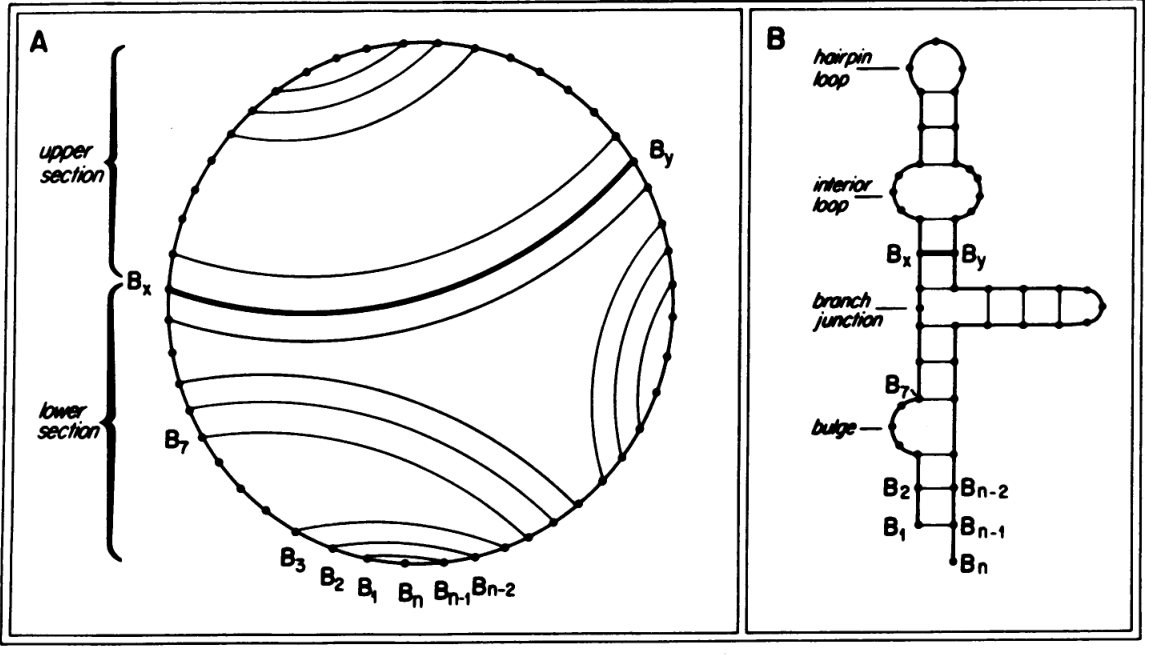
\includegraphics{nuss_rna}}
\end{center}
\caption{RNA secondary structure as described in the Nussinov algorithm.
Taken from the original publication \cite{nussinov1980fast}.}
\label{nuss_rna}
\end{figure}



Because of its dynamic programming
nature, this algorithm performs recursive decompositions of the RNA, building
larger structures out of repeated substructures. A natural representation of this is
depicted in Figure \ref{nuss_rna}. Part A of Figure \ref{nuss_rna} shows bonds as arcs across a circular
graph. In it, we see the nested nature of the structures being explored by the
Nussinov algorithm. Part B shows how these structures translate to actual RNAs in vivo. It also introduces the standard decompositions
of secondary structures, namely the hairpin loop, the interior loop, and the branch
junction or multiloop. Unlabelled in the diagram are stems; these are stacked
base pairings, for example $B1$, $Bn - 1$ and $B2$, $Bn - 2$.


\begin{equation} \label{eq:nuss_eq}
	M(i, j) = \max \left\lbrace A, B, C, D \right\rbrace 
\end{equation}
\[
A = M(i, j-1)
\]
\[
B = M(i+1, j)
\]
\[
C = M(i+1, j-1) + W(i, j)
\]
\[
D = \max \left\lbrace M(i, k) + M(k+1, j) \right\rbrace \: when \: i < k < j
\]



The recurrence relation for the Nussinov algorithm is defined in Equation \ref{eq:nuss_eq}. The first two cases ($A$ and $B$) find the score associated with not allowing the bases corresponding to indexes $i$ and $j$ to bond. Case $C$ conversely determines the score given that $i$ and $j$ are bonded. The final case $D$ computes the score associated with a bifurcation. A bifurcation here means decomposition of the RNA into two separate structures. This recurrence relation implies a $O(N^3)$
worst case time complexity and a $O(N^2)$ space complexity, as a $O(N^2)$ state space (all combinations of $i$ and $j$) is explored
with a linear time recurrence relation. In the original algorithm a constant ($p = 3$) was introduced that indicated the minimum size of a hairpin loop, as real RNAs typically do not have hairpin loops of fewer bases. The recurrence relation presented here has also been modified for the sake of clarity (cases $A$ and $B$ can be merged into case $D$) but the logic of the algorithm is equivalent.


This algorithm can also be extended to accommodate a more advanced energy
model. Instead of weighting each bond equally, bonds can be weighted
according to the proportion they are expected to contribute to the molecule's
stability \cite{nussinov1980fast}. When considering the value of a bond, it might be given greater
weight if it adds to the formation of a stem (a stabilizing structure), or
given lower weight if it forms an internal loop or bulge, as these generally
destabilize RNA molecules \cite{nussinov1980fast}. Unfortunately it is hard to find good values for
such weights, and determining which substructure a bond contributes to requires
backtracking in the modified algorithm presented by Nussinov \& Jacobson.

The reader should note that the Nussinov algorithm is old technology, and is no longer used for the prediction of RNA secondary structures. I have presented it in detail here because it forms the basis for the Zuker algorithm, which will now be discussed in detail.


\subsection{The Zuker Algorithm}

Soon after the work of Nussinov \& Jacobson, Zuker \& Stiegler \cite{zuker1981optimal}
described an altered version of the same algorithm which, instead of maximising
base pair weights, minimized the free energy of secondary structures. This is done
by introducing a number of thermodynamic rules for canonical structures like
hairpin loops, internal bulges, multiloops, unbonded base pairs, and stacked base
pairs. The algorithm is similar to the Nussinov algorithm, but requires another mutually recursive dynamic programming recurrence to inject
a relatively comprehensive thermodynamic scoring system. The original thermodynamic scoring scheme is borrowed from the work of Studnicka et al. \cite{studnicka1978computer} who presented a
complex but theoretically similar algorithm, albeit with
much worse asymptotic and implementation complexities. 


\begin{figure}
\begin{center}
\scalebox{0.27}{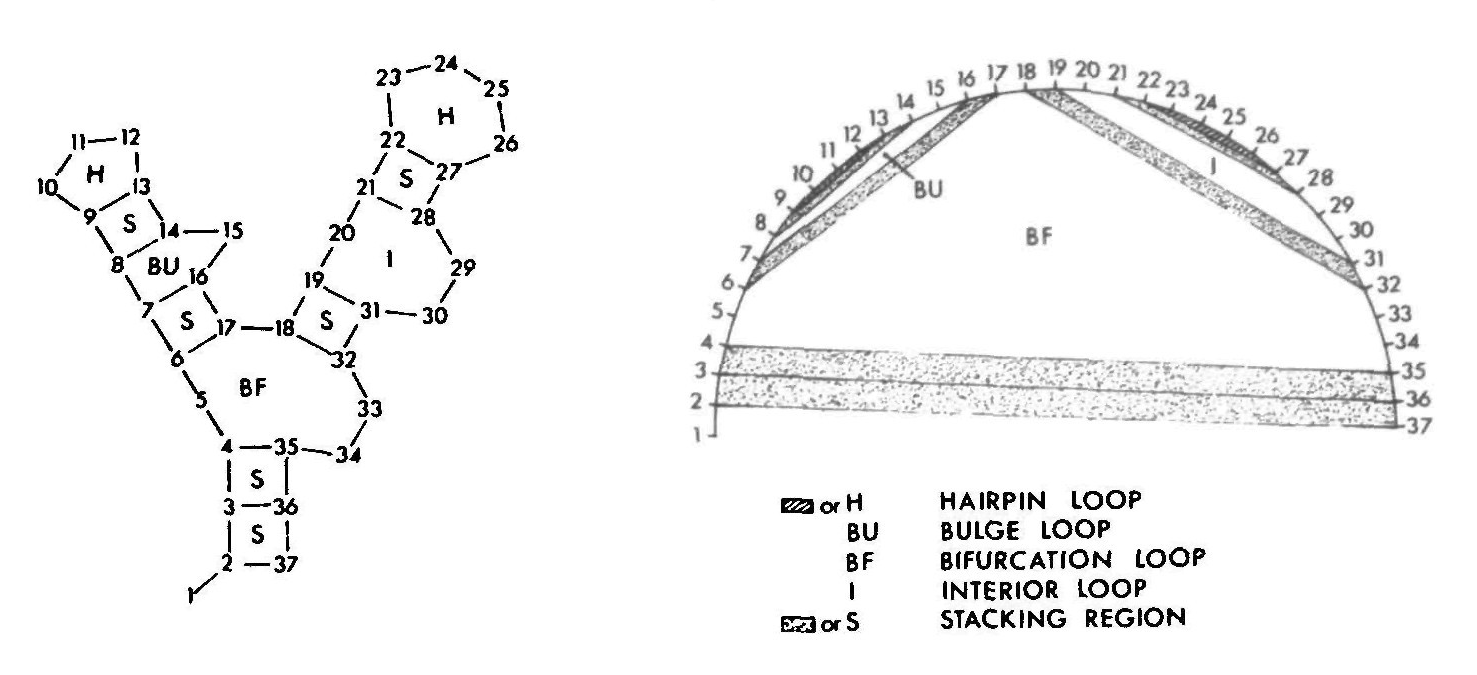
\includegraphics{figure4}}
\end{center}
\caption{Diagram of faces used in the Zuker algorithm. Taken from original
publication \cite{zuker1981optimal}.}
\label{zuk_struct}
\end{figure}

First I shall introduce some useful terminology which should clarify aspects of Zuker \& Stiegler’s
algorithm. The bases of an RNA molecule can be thought of as vertices in a planar graph. Edges between such vertices may then be represented as chords on a semicircular diagram (see Figures \ref{nuss_rna} and \ref{zuk_struct}). These chords are not allowed to touch. A chord
is admissible if it represents a chemically valid bond, and an
admissible structure is a structure whose graph contains only admissible bonds.
Thence, one can define a face of such a graph as any planar region bounded on all
sides. The
folding algorithm of Zuker \& Stiegler considers such faces as the basic contributing factor to a molecule's stability, unlike the algorithm of Nussinov \& Jacobson
which considers only individual bonds.


Let $E(F)$ represent the energy of a face $F$; impossible structures are given
an energy value of infinity, for example, hairpin loops smaller than three bases. In addition let $V(i, j)$ be defined as the minimum free
energy given that bases $i$ and $j$ are bonded, and let $W(i, j)$ represent
the minimum free energy of all structures contained within bases $i$ and $j$ inclusive.
Note that for $W(i, j)$ there need not be a bond between bases $i$ and $j$. Also,
if $i$ and $j$ cannot bond then $V(i, j) = \infty $. Finally note that $FH(i, j)$ represents a
hairpin loop structure from $i$ to $j$, and that $FL(i, j, i' , j' )$ is defined as the face bounded by the bonds $i, j$ and $i', j'$. Examples of these decompositions are shown
diagrammatically in the right half of Figure \ref{zuk_struct}. The labelled regions show faces
in a semicircular graph representing a strand of RNA. In the accompanying left
half of the figure, the same RNA structure is shown as it would appear in a real
RNA rather than in a purely diagrammatic depiction.

\begin{equation} \label{eq:zuk_v1_eq}
V(i, j) = \min \left\lbrace E1, E2, E3 \right\rbrace
\end{equation}
$$E1 = E(FH(i, j))$$
$$E2 = \min \left\lbrace E(FL(i, j, i', j')) + V (i', j') \right\rbrace \: where \: i < i' < j' < j$$
$$E3 = \min \left\lbrace W (i + 1, i') + W (i' + 1, j - 1) \right\rbrace \: where \: i + 1 < i' < j - 2$$


As shown by the definition provided in Equation \ref{eq:zuk_v1_eq}, $V (i, j)$ is computed by minimizing
three cases. The first case considers the bond between $i$ and $j$ closing off a hairpin
loop (H in Figure \ref{zuk_struct}). The second accounts for situations in which the bond from $i$ to $j$ results in a bulge (BU in Figure \ref{zuk_struct}), internal loop (I in Figure \ref{zuk_struct}), or the continuation of a stacking region with the
interior bond $i',j'$ (S in Figure \ref{zuk_struct}). The third and final case considers possible bifurcations contained within the bond between $i$ and $j$ (BF in Figure \ref{zuk_struct}).

\begin{equation} \label{eq:zuk_v1_eq2}
W (i, j) = \min \left\lbrace W(i + 1, j), W(i, j - 1), V(i, j), E4 \right\rbrace
\end{equation}
$$
E4 = \min \left\lbrace W (i, i') + W (i' + 1, j) \right\rbrace \: where \: i < i' < j - 1
$$

Equation \ref{eq:zuk_v1_eq2} is the recurrence for $W(i, j)$ as described by Zuker \& Stiegler.
Again there are three cases. The first two cases, $W (i + 1, j)$ and $W(i, j - 1)$,
should be thought of as a type of case in which possibilities having no bond between $i$ and $j$ are considered. This is similar to cases $A$ and $B$ from the Nussinov algorithm (Equation \ref{eq:nuss_eq}). The third case considers taking the bond from
$i$ to $j$. The fourth and final case allows for bifurcations in which two bonding regions split
the structure into two sections. The final minimum free energy of the best structure is defined by $W(1, n)$, where $n$ is the length of the RNA molecule. It should
be noted that the free energy for small molecules (fewer than 6 nucleotides in length) can easily be
precomputed, and forms the base case of the given recurrence relations. Because of
its efficiency ($O(N^3)$ time and $O(N^2)$ space), robustness, and extensibility, this method is,
even today, still the most popular available. The most widely used packages for RNA secondary structure prediction all contain implementations of the Zuker algorithm. Some notable examples are RNAfold from the Vienna RNA Package \cite{lorenz2011viennarna}, Zuker's own implementation Mfold \cite{zuker2003mfold}, and the recently updated RNAstructure \cite{bellaousov2013rnastructure}. The Zuker algorithm suffers a major shortcoming, however. Because all bonding regions are assumed to be nested, it
cannot handle the case of `pseudoknots'. 


\section{Pseudoknots}

Pseudoknots are structures in which a bonding pair may have its first
base inside another bonding pair, and the other base outside said bonding pair.
In short, it is not properly nested. These structures are not common,
but have been experimentally verified in numerous RNAs \cite{taufer2009pseudobase}. Additionally, pseudoknots also appear to perform useful biological functions. For
example, pseudoknots have been shown to allow frame shifting during translation
of proteins \cite{namy2006mechanical}. In layman’s terms, pseudoknots can change the way RNA is read
when being translated into protein. Frame shifting is used extensively by
viruses, particularly HIV \cite{namy2006mechanical}. Unfortunately, the problem of finding optimal
structures with pseudoknots has been shown to be NP-Complete \cite{lyngso2000rna}. In my investigation I did not consider the prediction of pseudoknotted RNAs as they are uncommon and difficult to model. However, I deem it important to understand how such structures could be integrated into the algorithms presented in this paper. As such, I have included a brisk overview of pseudoknot prediction techniques.

Despite the problem being NP-Complete, in 1999 Rivas \& Eddy \cite{rivas1999dynamic} introduced an ingenious dynamic
programming algorithm based on a new thermodynamic model encompassing pseudoknots. Their algorithm could predict a large (but incomplete) set of pseudoknot classes using
$O(N^6)$ time and $O(N^4)$ memory. They generalised the Zuker method by using a gap matrix to represent multiple regions being considered for bonding, rather than
the single continuous region used in the Zuker method. Because of its extreme
space and time requirements this algorithm is used only sparingly in practice; other thermodynamic based methods for pseudoknot prediction have
been formulated using similar principals. Deogun et al. \cite{deogun2004rna} described an algorithm which could handle a restricted class of pseudoknots (only those containing
non-recursive pseudoknots) in $O(N^4)$ time and using $O(N^3)$ space. Shortly after which Reeder \& Giegerich \cite{reeder2004design} presented an algorithm that could predict
only simple recursive pseudoknots that met their `canonization' criteria, and which required $O(N^4)$ time and $O(N^2)$ space. While
seemingly restrictive, this did, in fact, predict a large array of pseudoknots accurately. 

In recent years different approaches have been explored. In 2010 Sperschneider \& Datta introduced DotKnot \cite{sperschneider2010dotknot}, which improved upon previous algorithms by using probability dot-plot guided heuristics, and an updated energy model, to predict pseudoknots. DotKnot was able to predict pseudoknots more accurately than existing methods with more frugal space and time requirements. This technique was later refined so that it could predict H-type pseudoknots and intramolecular kissing hairpins \cite{sperschneider2011heuristic}.


\section{Accuracy}
\label{sec:accuracy}
It is important to test and compare the accuracy of various prediction methods.
As such, well established techniques have been developed over
the history of RNA structure prediction. Usually accuracy is determined by comparing predicted structures to known
structures. True Positives ($TP$) is defined as the number of base pairs which appear in both the predicted structure and the actual structure. False Positives
($FP$) is the number of predicted base pairs not in the true
structure \cite{lorenz2011viennarna}. Similarly, False Negatives ($FN$) is defined as the number of base
pairings in the reference structure but not present in the predicted structure \cite{lorenz2011viennarna}.
Sensitivity, also called the True Positive Rate ($TPR$), can be defined using the previously introduced values. I have given a mathematical definition of the $TPR$ in Equation \ref{eq:tpr}.

\begin{equation} \label{eq:tpr}
 \frac{TP}{TP + FN}
\end{equation}

Precision, also known as Positive Predictive Value ($PPV$), can also be calculated
using these values (see Equation \ref{eq:ppv}).


\begin{equation} \label{eq:ppv}
 \frac{TP}{TP + FP}
\end{equation}

RNAfold \cite{lorenz2011viennarna} is one of the leading RNA folding algorithms, and is made available
as part of the Vienna RNA package \cite{lorenz2011viennarna}. At its heart, it is an implementation
of the original dynamic programming algorithm first discovered by Zuker, albeit
with a more refined energy model. It is an extremely efficient implementation of
this algorithm, and is also one of the most accurate in terms of sensitivity and
PPV as compared to other implementations of the same algorithm \cite{lorenz2011viennarna}. When
Reeder \& Giegerich \cite{reeder2004design} first described their algorithm (implemented in the package pknotsRG) for pseudoknot prediction they compared it to RNAfold, and the
algorithm of Rivas \& Eddy (implemented in the same package and hereafter
referred to as pknotsRE) \cite{rivas1999dynamic}. 

Their algorithm generally had higher sensitivity than
both other methods, but it is worth noting that pknotsRE was extremely close
despite being based on an outdated energy model. This is possibly explained by
the fact that it is a more general, and thus a more powerful algorithm. RNAfold
lagged behind pknotsRE and pknotsRG in sensitivity, but executed orders of magnitude faster. Indeed, it has been shown to have excellent accuracy for smaller RNAs containing
no pseudoknots while also exhibiting unrivalled computation speed \cite{lorenz2011viennarna}.


\section{Locally Optimal Structure Prediction}
\label{sec:locopt}


DNA sequences, unlike typical RNA sequences, are very large indeed. Usually
on the order of hundreds of megabytes of data. DNA sequences often contain subsequences that code for RNAs. Functionally important RNAs typically have
a recognizable secondary structure. When searching a large genome for functional RNAs, one can use a sliding window of fixed size to find locally optimal
structures (see Figure \ref{fig:slidingwindow}). This can be done by running a typical cubic time implementation of the Zuker algorithm at every window location. Let $L$ be defined as the chosen
window size, and $N$ represent the length of the genome. This leads to a total complexity of $O(NL^3)$. While not prohibitive, this becomes intractable for many
genomes, which are typically extremely large---millions or billions of bases. 


\begin{figure}
\begin{center}
\scalebox{0.3}{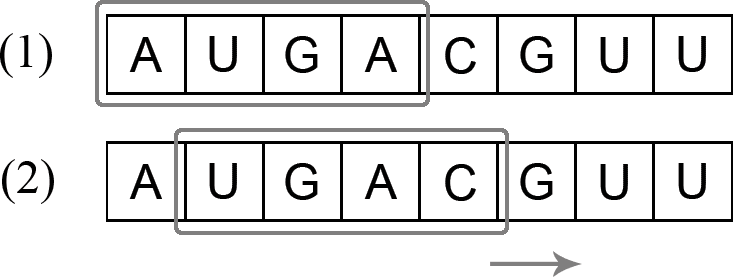
\includegraphics{slidingwindow}}
\end{center}
\caption{Depiction of how sliding windows can explore an RNA sequence.}
\label{fig:slidingwindow}
\end{figure}

In 2004, Hofacker, Priwitzer, and Stadler \cite{hofacker2004prediction} provided an excellent insight, and were
able to lower this bound to $O(NL^2)$. It was now possible to scan large genomes
for interesting RNA secondary structure motifs. This was achieved by modifying the Zuker algorithm. Specifically, the dynamic programming table from the previous step was used to quickly fill the table for
the next window in quadratic time; because consecutive windows overlap, preceding information can be meaningfully used in each forward computational step.
As a result it requires only a single table of size $O(L^2)$, and as such its memory complexity is only $O(N + L^2)$. Later, in 2009, Horesh et al. \cite{horesh2009rnaslider} managed
to lower the expected time bound to $O(NL)$ under the assumption that one is
folding RNAs that are typical of naturally occurring sequences. This average case time complexity was experimentally verified, as their algorithm was shown to outperform that of Hofacker, Priwitzer, and Stadler. 

Clearly good algorithms are
available for the folding of consecutive RNA windows. For even modest sized
RNAs, such algorithms are orders of magnitude faster than holistic secondary
structure prediction algorithms. However, this comes with the major caveat of not actually predicting
a complete secondary structure, but only a set of locally optimal structures.


\section{Context Free Grammars}
RNA sequences and their secondary structures can be represented as Context Free
Grammars (CFGs). Various production rules output different internal structures (such as
hairpin loops, or internal bulges) as symbols, with the terminals being the bases A, U, G,
and C. This is a fundamentally different approach to those discussed previously,
however CFGs can, in fact, use the same thermodynamic energy model. Stochastic Context Free Grammars (SCFGs) can be used to encode the plausibility of
production rules, and thus find the most plausible parse tree using a thermodynamic model \cite{rivas2012range}. In addition, these kinds of algorithms can be trained to
incorporate statistical information such as phylogenetic similarity, or machine
learned parameters \cite{rivas2012range}. These kinds of methods have trouble with pseudoknots, as non-nested structures are not compatible with CFGs.
A notable workaround was applied by Kato, Seki, and Kasami \cite{kato2006stochastic}, who used
multiple context free grammars to model pseudoknots. However, their approach
increases time and space requirements prodigiously.


The greatest strength of context free grammar based approaches is that they
can diverge from the use of free energy minimisation entirely. This is advantageous as using
a physics based model---such as free energy minimization---requires a large volume
of experimentally verified parameters. For this reason, many parameters are often not included in such models because they cannot be quantified empirically.
The energy value of multi-branch loops, for example, is not known, and is usually
guessed in modern RNA prediction algorithms. Likewise, the inter-structural
interactions of hairpin loops, bulges, multi-branch loops, and internal loops has
not been quantified experimentally and is thus not used as a free energy parameter. CONTRAfold \cite{do2006contrafold} was one of the first SCFG based algorithms to achieve
comparable performance to Zuker-like free energy minimization methods. It does
away with the notion of free energy minimization altogether, and instead uses a
set of trained parameters based on conditional log-linear models. CONTRAfold
achieved an average prediction sensitivity higher than RNAfold \cite{lorenz2011viennarna}, and also higher
than that of Mfold \cite{zuker2003mfold}, an RNA prediction package similar to RNAfold.




\section{Soft Computing}
The use of soft computing techniques has also yielded some success in the prediction of RNA secondary structure. Koessler et al. \cite{koessler2010predictive} modelled RNA structures
as a tree of internal substructures, then used artificial neural networks to recognize
which of these trees appeared most RNA like. These trees are generated by constructing basic secondary structures and combinatorially merging them together
to form many trees, each of which is represented as a vector of simpler trees.
This vector is used as the input to the neural network. 

This kind of combinatorial blending of RNA stems is also a techniques shared by genetic algorithms. Indeed, this
is precisely the starting point of Van Batenburg, Gultyaev, and Pleij \cite{van1995apl}, who
used a simple genetic algorithm to predict secondary structure. Their algorithm
started by computing an array of all possible stems; each genome was represented
as a binary string where \texttt{1} indicates a stem is in the candidate structure, and \texttt{0}
indicates that it was not. Their genetic algorithm proceeded by seeding the genomes
with random bits, then in a series of generation steps performed typical binary
mutation, crossover, and breeding, conserving and selectively breeding the fittest
solutions. Fitness was defined in their algorithm as the summed length
(number of bonds) of all stems. In an improved version, the summed stacking
free energy reduction of all stems was used instead.

Unfortunately they discovered a problem with this approach: the population
contained a relatively large portion of zero fitness individuals. This is because
many combinations of stems are incompatible with each other, yielding impossible
structures. Instead of giving these structures zero fitness, they altered their algorithm slightly to disallow crossover for stems that create an invalid structure.
In addition to this, they also explored an important advantage of genetic algorithms for RNA secondary structure prediction: that of kinetic folding. Kinetic
folding is the hypothesis that some RNAs, particularly large ones, have a rugged
energy landscape, and because of the incremental process of transcription and
folding (which happen simultaneously) become stuck in suboptimal areas during
folding \cite{treiber2001beyond, van1995apl}. 

The algorithm of Van Batenburg, Gultyaev, and Pleij simulated
this process by limiting the size of stems that could contribute to a genome, and
increasing this size over time until the length of the RNA was reached. This
single modification to their algorithm yielded the greatest improvement in predictive power. It should also be noted that it can predict pseudoknots, as
the algorithm does not force stems to be nested. Despite this, their approach was
still less accurate than the dynamic programming approaches they compared it
to. This is likely because their energy model was puerile in comparison, rather than because the algorithm is flawed.

Indeed, Wiese, Deschenes, and Hendriks \cite{wiese2008rnapredict} introduced an improved
genetic algorithm based on the same principles as that of Van Batenburg, Gultyaev,
and Pleij, but instead using an advanced energy model for fitness. They then
demonstrated that it outperforms the popular dynamic programming algorithm
Mfold \cite{zuker2003mfold}, which uses a similarly complex model. Wiese, Deschenes, and Hendriks noted that as the length of RNA molecules increases, the correlation between lower free energy and accuracy decreases. They concluded that this was due to the incompleteness of the current thermodynamic model of RNA folding. Unlike the algorithm of Van Batenburg, Gultyaev, their algorithm is oblivious to kinetic folding, and does not attempt to simulate it.

\section{Kinetic Folding}
Kinetic folding is not a purely notional thesis. It has been observed in vivo, and evidence has existed since the early 80s. Kramer \& Mills \cite{kramer1981secondary} reported seeing preliminary secondary structures form, break apart, and reform into other structures during transcription. This means that as RNA is synthesized, its structure is already undergoing dynamic formation with every additional nucleotide. Over a decade later Morgan \& Higgs \cite{morgan1996evidence} examined many RNA molecules and found that typical structures had suboptimal free energy. They postulated that this was due to kinetic folding, and that errors in the free energy parameters of the current model could not fully explain the discrepancy. Recently Proctor and Meyer \cite{proctor2013cofold} improved secondary structure perdition accuracy by simulating kinetic folding. The effects of kinetic folding were captured using a scaling function which weighted closer nucleotides more than distant nucleotides. Proctor and Meyer \cite{proctor2013cofold} reported that this improved prediction accuracy; particularly for RNA molecules comprising greater than 1000 nucleotides. 


\section{State of the Art: Global Optimization}
\label{sec:softa}
Most current state of the art algorithms fold RNA in a way that globally maximises score according to some model. The Zuker algorithm, for example, finds the global minimum free energy configuration. SCFG based algorithms maximise the probability of a parse tree. This bias is largely due to the `Thermodynamic Hypothesis'. Anfinsen \cite{anfinsen1973principles} presented this hypothesis as the underlying principle for the formation of biologically active proteins. He held that proteins fold into a minimum Gibbs free energy conformation in their typical biological environment. (Environment being defined as the molecules physiological state: pH, temperature, and ion concentration.) Furthermore, through natural selection, molecules that are most likely to fold into the correct shape have evolved. Therefore we should be able to determine the structure of biologically active molecules (particularly proteins in Anfinsens original thesis) by finding a minimal free energy conformation, given the building blocks of the molecule. This insight has been invaluable for folding proteins and RNAs in silico. Despite this, it has recently become clear that methods for the prediction of RNA secondary structures have hit an upper limit in accuracy.

In her discussion of modern RNA prediction, Rivas \cite{rivas2013four} unified pseudoknot-free RNA folding algorithms. Her core observation is that all such prediction algorithms contain the same four key components: an architecture, or the production rules of a grammar; a scoring scheme, or how scores are assigned to these production rules; and the parametrization of the scoring scheme, or the specific values assigned to it. These features are referred to by Rivas, and by myself in the following discussion, as the `model'. The fourth and final feature is the folding algorithm used to find the best structure given the model. Here Rivas notes that the two dominant folding algorithms are interchangeable. The Cocke-Younger-Kasami (CYK) algorithm, used to parse SCFGs, and free energy minimizing algorithms based on the work of Zuker are isomorphic for the purpose of parsing RNA grammars. Rivas additionally notes that all scoring schemes and parametrizations appear to hit an accuracy upper limit, and that complex, machine learned models are only slightly more accurate than thermodynamic models. In fact, relatively basic grammars with hundreds of parameters seem to perform almost equivalently to those with tens of thousands. While Rivas managed to unify many aspects of RNA prediction she did not recognise that all such algorithms are based on those same assumptions underpinning the thermodynamic hypothesis: they seek to globally maximise a scoring function for the final RNA secondary structure. 

I propose that, in RNA molecules, local interactions are stronger than global interactions. As a result RNA molecules will misfold into a global structure made up of locally optimal structures. This is my core hypothesis. If this assumption is correct it follows that there exists a set of `windows' that, when folded using any reasonable model, will be more accurate than the corresponding global optimum using the same model. There is already some evidence for this hypothesis. Dawson et al. \cite{dawson2013new} used variable Kuhn lengths to accurately predict RNAs containing less than 100 nucleotides. Kuhn length is the size of a segment in a polymer chain. It is a simplifying assumption that allows one to treat the entire chain as a sequence of Kuhn segments. In addition, Dawson et al. showed that the energy landscape of these RNAs, when the correct Kuhn length was applied, was funnel shaped. Without such simplifying assumptions the energy landscape of RNAs is notoriously rugged, with in vivo secondary structures often becoming `trapped' in suboptimal states; this is most apparent in large RNAs \cite{ditzler2008rugged}.

If my hypothesis is supported, I aim to leverage the insights provided to improve the accuracy and speed of RNA secondary structure prediction.

\chapter{Methodology}

\section{Materials}
\subsection{Environment}
All algorithms were implemented and tested using Ubuntu 13.10 running on an Intel i5-3210m processor with four gigabytes of RAM. The GNU C compiler (GCC) version 4.8.2 was used to compile all C and C++ code. 

\subsection{Software}
The Vienna RNA Package \cite{lorenz2011viennarna} was used as a base for all algorithms presented in this paper. This package contains many useful programs for working with RNA. The RNAfold and RNALfold modules were used in this investigation. 

RNAfold is a modern implementation of Zuker's folding algorithm. It predicts the minimum free energy secondary structure of an RNA given the primary sequence. It can also calculate the Boltzmann partition function, producing a matrix of base pair probabilities. Additionally the RNAfold tool can compute the energy of any arbitrary secondary structure, given a corresponding RNA primary sequence, under it's thermodynamic energy model.

The RNALfold module implements a sliding window RNA folding algorithm. It is designed to find all locally optimal secondary structures for an RNA of size $n$, using a window of fixed size $L$. RNALfold implements Hofacker, Priwitzer, and Stadler's algorithm \cite{hofacker2004prediction}, and thus uses $O(nL^2)$ time and $O(n + L^2)$ space. I note here that this is not the most optimal algorithm available. As I have discussed in section~\ref{sec:locopt}, Horesh et al. \cite{horesh2009rnaslider} presented an algorithm that also folds consecutive windows using a similar model. However, they achieved a typical time complexity of $O(nL)$. This algorithm was not used because the implementation give by the authors is based on an older energy model taken from the Mfold \cite{zuker2003mfold} package. RNALfold is based on the same energy model as RNAfold, which has been recently updated \cite{lorenz2011viennarna}. For the sake of accurate comparison to RNAfold, and to ensure a state-of-the-art energy model, RNALfold was used.

Version 2.1.6 of the Vienna RNA package was used. The package was built from the C source code after minor modifications were made to the RNALfold module. The Vienna RNA makefile was used to compile the package. The makefile compiles numerous standalone console applications for Vienna RNA's modules. It also creates a static library called RNAlib. This library was linked at compile time, and used to call RNAfold and RNALfold from the algorithms I shall subsequently describe.

The \texttt{Lfold.c} and \texttt{Lfold.h} files (which RNALfold comprises) were modified so that, when the algorithm was executed, RNALfold returned a linked list of local secondary structures and their free energy. Before modification it would instead print them to the standard output stream. The modified versions of these files are available in the files associated with this report.

Statistical tests, regression analyses, and plots were generated using GNU Regression, Econometrics and Time-series Library (as called `gretl') version 1.9.14.


\subsection{Testing Set}
The RNA secondary structures used to test algorithms presented in this paper were taken from the RNA STRAND database \cite{andronescu2008rna}. The RNA STRAND database is a free-to-use, curated collection of RNA secondary structures taken from various publicly available databases and publications. A subset of RNA structural data was extracted from the database. This subset contained only RNA structures that were marked having been verified using X-Ray Crystallography, or Nuclear Magnetic Resonance imaging. It also comprises only whole RNAs; none of the RNAs used were fragments or subsequences of larger RNA molecules. Finally, no duplicates were allowed in the selected set. Hereafter, I shall refer to this collection of RNA secondary structures as the `testing set'. The testing set contained 392 different RNA molecules ranging in length from 20 to 3032 nucleotides.


\section{RNA Intervals}
Running an algorithm which generates consecutive windows of size $L$ over a RNA primary sequence of size $n$ will produce $n-L$ windows of size $L$. Each of these windows may contain one or more discrete structural element. For example, a window may contain two disjoint stems. After generating these windows, a post-processing step was executed in which any such disjoint secondary structural elements were split up. While RNALfold does this without modification, it might be necessary to encode this manually using a different implementation.

\begin{figure}
\begin{center}
\scalebox{0.35}{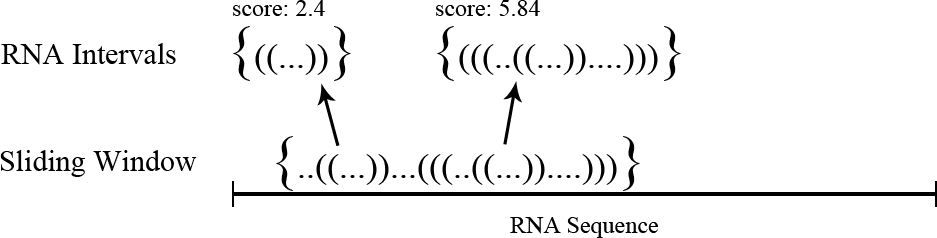
\includegraphics{rnainterval}}
\end{center}
\caption{The relationship between a sliding window and it's RNA intervals. RNA secondary structures are represented using dot-bracket notation.}
\label{fig:rnainterval}
\end{figure}

Once all disjoint structural elements were split up, they were assigned a score. This score was proportional to their free energy reduction. I call this pair of stem and score an `RNA interval'. Every window generated using a sliding window algorithm was processed into a collection of RNA intervals. A window may contain none or many RNA intervals depending on the density of stems.





\section{Merging RNA Intervals}
\label{sec:merging}

Given an RNA sequence, it is easy to generate a set of RNA intervals by running any sliding window algorithm, and storing the RNA intervals generated for each window. Many of these intervals will overlap, or contain fragments of one-another. To construct a plausible and complete secondary structure for the original RNA out of these intervals, a procedure must select a subset of the RNA intervals generated this way. I devised several methods for doing this. The goal of an RNA interval merging algorithm is to produce a valid secondary structure out of a set of RNA intervals which is as accurate (compared to the actual secondary structure) as possible.


Let $W$ be the set of all RNA intervals to choose from, and let the set $S$ represent the set of selected intervals. Also, an interval is compatible with another if they do not overlap and neither interval contains the other (see Figure \ref{fig:compatible}. Taking only mutually compatible intervals will result in a valid RNA  structure. The way in which these intervals are selected determines the accuracy of the resulting structure.

\begin{figure}
\begin{center}
\scalebox{0.35}{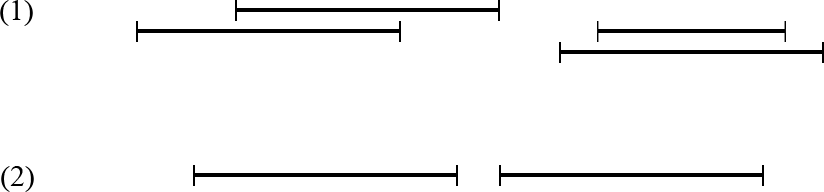
\includegraphics{compat}}
\end{center}
\caption{Case 1 shows RNA intervals that are not compatible. Case 2 shows an example of compatible intervals.}
\label{fig:compatible}
\end{figure}

If any RNA merging algorithm can find RNA secondary structures which are consistently more accurate than those generated by conventional prediction algorithms, my hypothesis would be supported. This is because such an algorithm builds final structures out of a collection of locally optimal substructures.

\subsection{Top-Down Selection}
In this method, $W$ is sorted by RNA interval size in descending order. The algorithm then examines each element of $W$ in order. If an element of $W$ is compatible with all elements of $S$, it is added to $S$.

\begin{algorithm}
  \caption{Top-Down Selection}
  \label{tds}
  \begin{algorithmic}[1]
  \State Let $W$ be the set of RNA intervals
  \State Let $S$ = \{\}
  \State \Call {Sort}{$W$}
  \ForAll{$W$ as $e$}
  	\If {\Call{Compatible}{$e$, $S$}}
  		\State $S = S \cup e$
  	\EndIf
  \EndFor
  \State \Return $S$
  \end{algorithmic}
\end{algorithm}

	
The algorithm (see Algorithm \ref{tds}) examines every element of $W$ exactly once, and for each element checks for compatibility with $S$. The naive way to check for compatibility is to examine every element in $S$. This would give the algorithm a worst case time complexity of $O(n^2)$, where $n$ is the number of intervals, as all the intervals in $W$ may be mutually compatible. This is a result of the algorithm first checking $S$ of size \texttt{0}, then 1, up to $n-1$, totalling $(n-1)((n-1)+1) / 2$ steps. Additionally it requires $O(n)$ space to store $S$.

It is possible to lower the time complexity to $O(n \log n)$ by storing the elements of $S$ in an augmented interval tree. Querying this tree finds any elements of $S$ that intersect the interval in question. This query takes $O(\log n)$ time and is executed $n$ times---once for every element of $W$. This is optimal, since the \texttt{Sort} operation requires $O(n \log n)$ time. Hence, the final worst case time complexity is $O(n \log n)$ and the final worst case space complexity is $O(n)$.


\subsection{Bottom-Up Selection}
This algorithm is identical to Top-Down Selection, except that $W$ is sorted by interval size in ascending order.

\subsection{Score Selection}
This algorithm is identical to Top-Down Selection, except that $W$ is sorted by score in descending order.


\subsection{Weighted Activity Selection}

\begin{figure}
\begin{center}
\scalebox{0.35}{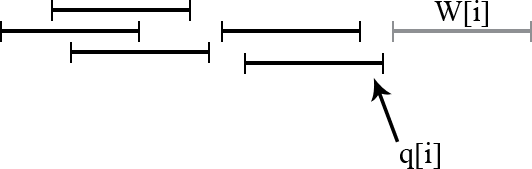
\includegraphics{q-i}}
\end{center}
\caption{The interval stored in $q[i]$ for the RNA interval $W[i]$.}
\label{fig:rightcompat}
\end{figure}

The weighted activity selection problem is a generalization of the activity selection problem. Given a set of intervals, each of which is assigned a weight, the problem is to find a subset such that none of these intervals touch one-another, and the sum of their weights is maximised. This maps naturally to the problem domain of this investigation. I used this algorithm to find the subset of compatible windows which have the minimum sum free energy, or put another way, maximum score.

\begin{algorithm}
  \caption{Weighted Activity Selection}
  \label{was}
  \begin{algorithmic}[1]
  \State Sort $W$ by right end points
  \State Let $n$ = $|W|$
  \State Let $q$ = array[$1..n$]
  
  \For{$i = 1 \to n$}
  	\State $q$[$i$] = highest index $< i$ which is compatible with $i$
  \EndFor
  \State Let $dp$ = array[$0..n$]  
  \State $dp$[0] = 0
  \For{$i = 1 \to n$}
  	\State $dp$[$i$] = $\max (weight[i] + dp[q[i]], \: dp[i-1])$
  \EndFor
  \State \Return $dp[n]$
  \end{algorithmic}
\end{algorithm}

The initial sort (see line 1 in Algorithm \ref{was}) requires $O(n \log n)$ time. In the following loop (line 4) the algorithm finds the right most element in $W$ such that it is compatible with element $i$ (see Figure \ref{fig:rightcompat}). This can be done using a binary search. Hence the total worst case run time of the loop is also $O(n \log n)$. The final dynamic programming array fill (line 9) requires only $O(n)$ time. As a result the final time complexity of this algorithm is $O(n \log n)$. Additionally, $O(n)$ space is required for the arrays $q$ and $dp$.


\subsection{Comparison of RNA Interval Selection Algorithms}

The reader should note that all presented selection algorithms have the same $O(n \log n)$ worst case time complexity, and the same auxiliary space complexity of $O(n)$. None of these algorithms have large constant factors. Therefore, my final choice of algorithm was based solely on the accuracy of the computed secondary structure.

In order to test and compare these selection algorithms, all the windows of size five to 500 were precomputed for every RNA in the testing set. This is to say that the sliding window algorithm was run for a window size of five, then size, up to and including size 500 for each RNA, and the resulting RNA intervals were cached. The minimum size of five was chosen because meaningful stems do not form with a size fewer than five nucleotides. The maximum of 500 was due to space and time constraints. Computing these windows took several days, and used 2.5 gigabytes of memory to store.

Each selection algorithm was run using these data as input. For every RNA, the single most accurate window size was recorded, along with the accuracy value. Accuracy was judged as the F-Score, which is the harmonic mean of sensitivity and precision (defined in Section \ref{sec:accuracy}).




\section{Prediction Using Windows}
\label{sec:absplat}
In this approach I computed sliding windows using a `splat' of sizes. Weighted Activity Selection was then done on the resulting set of computed RNA intervals. See Section \ref{sec:localopt} for an explanation of why Weighted Activity Selection was chosen. I explored several methods for finding good splats. I present here to most successful technique, which I call `$ab$-splat' prediction. Initially the algorithm started at a small window size, and exponentially increased the scope of the window until a threshold was exceeded. This is explained using pseudocode in Algorithm \ref{absplat}.

\begin{algorithm}
  \caption{$ab$-splat}
  \label{absplat}
  \begin{algorithmic}[1]
  \State Let $RNA$ be the primary RNA sequence being folded
  \State Let $i = a$
  \State Let $S = \{\}$
  \While{$i \leq $ \Call{Treshold}{$RNA$} }
  	\State $S = S \: \cup $ \Call{ComputeSlidingWindows}{$RNA$, $i$}
  	\State $i = i \times b$
  \EndWhile
  \State \Return \Call{WeightedActivitySelection}{$S$}
  \end{algorithmic}
\end{algorithm}

The \texttt{Threshold} function was defined as $\sqrt{ \texttt{RNA Length} } \times 9.5$. This formula was found using empirical experimentation.

\subsection{Time Complexity}

The time complexity of this algorithm is non-trivial to deduce. The runtime of \texttt{ComputeSlidingWindows} is $O(nL^2)$ where $L$ is the window size, and $n$ is the length of the RNA. It is called once for every window size. In addition \texttt{WeightedActivitySelection} uses $O(n \log n)$ time, where $n$ is the number of RNA intervals in the set $S$. I shall now show that $ab$-splat has a worst case time complexity of $O(n^2)$.

\begin{equation} \label{eq:abtimeone}
	n a^2 + n(a b)^2 + n(a b^2)^2 + n(a b^3)^2 + \cdots + n^2
\end{equation}

Equation \ref{eq:abtimeone} shows the number of steps required to run the sliding window algorithm for every window size in $ab$-splat. The second term represents $L^2$ for exponentially increasing $ab$ pairs. Clearly the worse case is where $L = \sqrt{n}$ and hence $L^2 = n$ leading to a largest computational cost of $n^2$. Factoring out $n^2$, we get Equation \ref{eq:abtimetwo}

\begin{equation} \label{eq:abtimetwo}
	n^2 ( \frac{n a^2}{n^2} + \frac{n(a b)^2}{n^2} + \frac{n(a b^2)^2}{n^2} + \frac{n(a b^3)^2}{n^2} + \cdots + 1)
\end{equation}

In the limit to infinity all terms except \texttt{1} tend toward zero. Hence we are left with a final time complexity of $O(n^2)$ for computing all required sliding windows. Now I shall show that this dominates the cost of running weighted activity selection.

Every window size produces $O(n)$ windows of size $L$. Every such window can contain at most $O(L)$ RNA intervals. Equation \ref{eq:intervalsone} shows the total number of RNA intervals produced. By factoring out $n^\frac{3}{2}$ in a similar manner to Equation \ref{eq:abtimetwo} described above, we see that the number of RNA intervals is $O(n^\frac{3}{2})$.


\begin{equation} \label{eq:intervalsone}
	n a + n(a b) + n(a b^2) + n(a b^3) + \cdots + n^\frac{3}{2}
\end{equation}

Weighted activity selection uses $O(n \log n)$ time. As we have $O(n^\frac{3}{2})$ windows in the worst case, this leads to a worst case time complexity of $O(n^\frac{3}{2} \log n^\frac{3}{2})$, which is dominated by $O(n^2)$. Computing the largest sliding window requires only $O(n)$ space, since it uses $O(L^2)$ space in all cases. Weighted activity selection will additionally require only $O(n^\frac{3}{2})$ space. As all of these RNA intervals must be stored in $S$, $ab$-splat will thus use $O(n^\frac{3}{2})$ memory in the worst case. In contrast, the Zuker algorithm requires $O(n^3)$ time and $O(n^2)$ space. The computational bottleneck is usually time, however. 

\subsection{Test Procedure}

A brute force method was used to test a combinatorial set of values for $a$ and $b$ such that $10 \leq a \leq 30$ and $1.5 \leq b \leq 4.0$. In this method, all integer values for $a$ were attempted, and values for $b$ were generated with a step size of \texttt{0.1}. This method was exhaustive, but slow. To speed up computation, precomputed window were used. This meant that the \texttt{Threshold} function had to be altered slightly, as only windows up to size 500 were precomputed:  $min(\sqrt{ \texttt {RNA Length } } \times 9.5, \: 500)$.

To test this algorithm, the testing set was randomly partitioned into two sets containing an equal number of RNAs. One of these sets I called the training set, the other I called the validation set. The aforementioned brute force search was done on the training set, and the F-Scores for $ab$ pairs was recorded; $ab$ pairs with highest F-Scores were deemed the best. These scores were then validated by running the same procedure on the validation set, then attempting to correlate the scores of $ab$ pairs between training and validation sets. This  indicated if high scores in the training set were related to high scores in the validation set. The correlation also allowed me to determine if results found in the training set were valid.

The best $ab$ pair was used to configure the $ab$-splat algorithm, which was then run on the full testing set, and it's F-Scores recorded. These F-Scores were then compared directly to F-Scores produced by RNAfold, which was also run on the full testing set. In addition to this, the time to execute each algorithm was recorded and compared. Precomputed windows were not used so that the runtime and accuracy could be fairly compared to RNAfold. Because of this, the standard \texttt{Threshold} function was used in this scenario.

\chapter{Results}

\section{RNA Interval Selection}
The purpose of the following tests was to determine if any RNA interval merging algorithms (see Section \ref{sec:merging}) could potentially achieve better accuracy than globally optimizing algorithms. The RNAfold package is a modern implementation of the Zuker algorithm, which globally optimizes a thermodynamic scoring scheme. RNAfold is thus used for comparison. I predicted that some merging algorithms should have higher accuracy if local interactions are stronger than global interactions during RNA folding.

The average score between all RNA interval selection algorithms was compared (see Table \ref{tab:summaryselection}). The highest scoring algorithm appeared to be Top-Down Selection, closely followed by Weighted Activity Selection, then by Bottom-Up Selection. To verify this performance gap, a Wilcoxon Signed-Rank Test was done to compare the recorded F-Scores for corresponding RNA. This test was chosen because the data recorded did not appear to be parametric. While this test reflected the small difference in averages between Weighted Activity Selection and Top-Down Selection ($z = 1.33066$, see Table \ref{tab:wilcoxonselection}), it was not statistically significant ($p > 0.001$). To further test Top-Down Selection and Weighted Activity Selection, another Wilcoxon Signed-Rank Test was done on only RNAs of length $\geq 300$ bases. This revealed a moderate, and statistically significant, difference, indicating that Weighted Activity Selection generally had higher F-Scores for larger RNAs ($p < 0.001, z = 4.55591$). Finally, a Wilcoxon Signed-Rank Test was done between Weighted Activity Selection and Score Selection to check for circular dominance. In accordance with the mean F-score values, Weighted Activity Selection appeared to have higher F-Scores than Score Selection ($p < 0.001, z = 12.0957$).

\begin{table}
\centering
\begin{tabular}{l*{6}{c}r}
Algorithm	& Mean & Median \\
\hline
BUS &  0.38122    &    0.35065   \\
SS & 0.68373    &    0.73098  \\
WAS & 0.70395   &     0.75709  \\
TDS & 0.71684   &     0.80000  \\
\hline
RNAfold & 0.57483    &    0.60870 \\
\end{tabular}

\caption{Summary statics of recorded F-Scores for Weighted Activity Selection (WAS), Top-Down Selection (TDS), Bottom-Up Selection (BUS), Score Selection (SS), and RNAfold.}
\label{tab:summaryselection}
\end{table}



A Wilcoxon Signed Ranks Test was also used to compare the best recorded F-Scores for all RNA interval selection algorithms, and those recorded for RNAfold (see Table \ref{tab:wilcoxonselection}). All tests were statistically significant ($p < 0.001$). All algorithms but Bottom-Up Selection were shown to outperform RNAfold; Weighted Activity Selection in particular ($z = 13.2082$). Figure \ref{fig:wasrnafold} depicts this performance difference clearly.


\begin{table}
\centering
\begin{tabular}{l*{6}{c}r}
Test Subjects	& $z$-value & Two-tailed $p$-value \\
\hline
WAS \& TDS 	& -1.33066 &	0.183301 \\
WAS \& TDS (RNA length $\geq 300$)	& 4.55591 &	$2.60801 \times 10 ^{-6}$ \\
WAS \& SS & 5.94681 &	$2.73418 \times 10^{-9}$  \\
\hline
BUS \& RNAfold & -9.13933 &	$6.28392 \times 10^{-20}$  \\
SS \& RNAfold & 12.0957 &	0  \\
TDS \& RNAfold & 13.119 &	0  \\
WAS \& RNAfold & 13.2082 &	0  \\
\end{tabular}

\caption{Results of Wilcoxon Signed-Rank Testing for F-Scores. Weighted Activity Selection (WAS), Top-Down Selection (TDS), Bottom-Up Selection (BUS), Score Selection (SS), and RNAfold are included.}
\label{tab:wilcoxonselection}
\end{table}


\begin{figure}
\begin{center}
\scalebox{1}{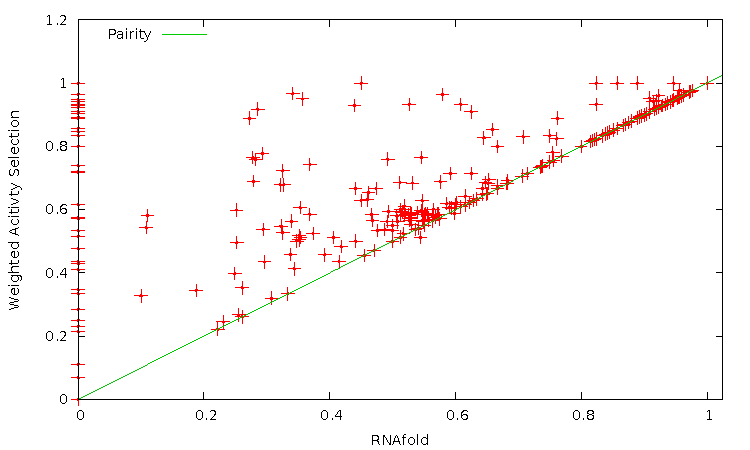
\includegraphics{wasrnafoldplot}}
\end{center}
\caption{F-Scores for matching RNA test cases achieved by Weighted Activity Selection and RNAfold plotted against one-another. The green line represents parity. Any points above the line are cases in which Weighted Activity Selection performed better, points below the line indicate that RNAfold was more accurate. Note that a maximum F-Score is \texttt{1.0}.}
\label{fig:wasrnafold}
\end{figure}


\section{Using RNA Intervals For Prediction}
\label{sec:res_absplat}
The purpose of the following tests was to determine if the $ab$-splat algorithm (see Section \ref{sec:absplat}) was more accurate than RNAfold. Additionally, further tests were done to compare the runtime efficiency of both algorithms. It was expected that $ab$-splat would be more accurate than, and run faster than, RNAfold.

An ordinary least squares linear regression was done to determine the correlation between F-scores recorded for $ab$-splat in the training and validation sets. Figure \ref{fig:abcorrelation} depicts the resulting model. A strong correlation was found ($R^2 = 0.703$, $p < 0.001$) for scores in the training set versus scores in the validation set. The best $ab$ value pair found in the training set was $a = 24$, $b = 1.8$. The $ab$-splat algorithm was configured using these values. As the data did not appear to be normally distributed, a Wilcoxon Signed-Rank test was done to compare F-scores for $ab$-splat (with the best $ab$ pair) and RNAfold. This test revealed a small difference in the F-scores in the population ($z = 0.1067$), which reflected the small difference in averages (mean RNAfold score = $0.57483$, $ab$-splat = $0.58588$). However, this discrepancy was not statistically significant ($p = 0.915021$).


\begin{figure}
\begin{center}
\scalebox{1}{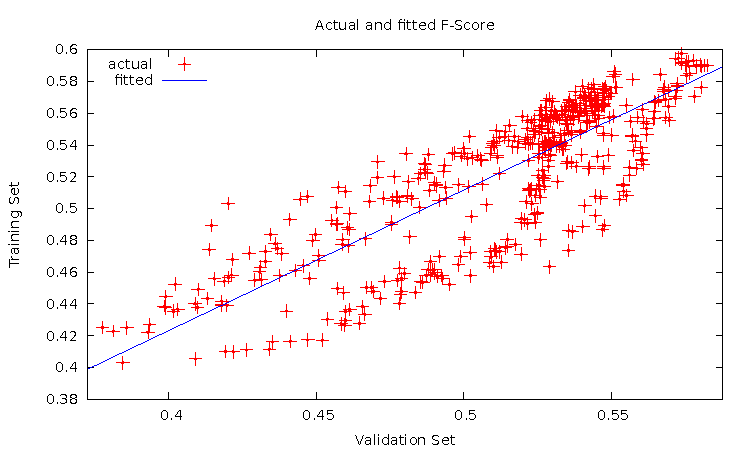
\includegraphics{abcorrelation}}
\end{center}
\caption{Correlation of F-Scores for $ab$-splat in training set versus validation set. R-squared value = 0.702901, $p$-value $< 0.0001$. Standard Error of Regression = 0.025032.}
\label{fig:abcorrelation}
\end{figure}



\begin{figure}
\begin{center}
\scalebox{1}{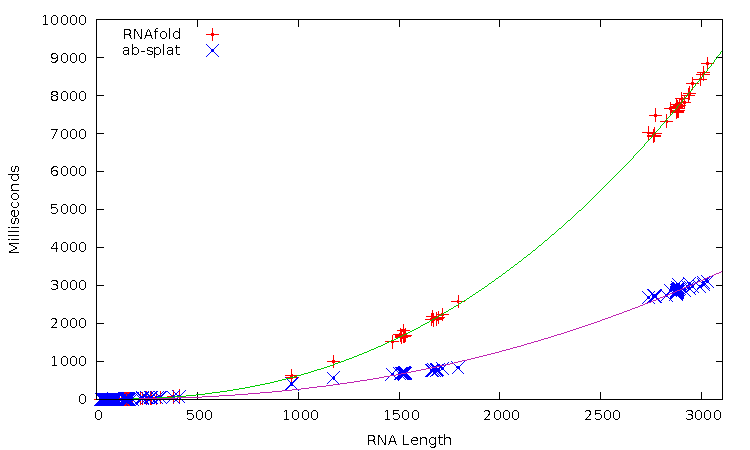
\includegraphics{zukerabtime}}
\end{center}
\caption{A comparison of the time taken for RNAfold to run, compared to $ab$-splat. This graph indicates how each scale with increasing RNA length. Best fit regression lines are also shown.}
\label{fig:zukerabtime}
\end{figure}

Simple empirical observation was used to compare the runtime of RNAfold and $ab$-splat. A graph representation of the observed times is shown in Figure \ref{fig:zukerabtime}. This graph shows how the runtime of these algorithms grow with increasing RNA length. Both appeared to have a polynomial curve. Further analysis showed that both were best approximated by a polynomial regression. Both regression equations indicated a strong relationship between RNA length and algorithmic runtime ($R^2 > 0.99$). The best fit regression line for RNAfold runtime was $O(n^{2.374})$ where $n$ is RNA length. The $ab$-splat algorithm has a best fit regression line that was $O(n^{2.25})$. A summary of the regression equations can be found in Table \ref{tab:algorithmtimeregression}.


\begin{table}
\centering
\begin{tabular}{l*{6}{c}r}
Algorithm	& Regression Equation & $R^2$ value \\
\hline
RNAfold &  $y=0.358+4.7 \times 10^{-5} \times x^{2.374}$    &    0.9997    \\
$ab$-splat & $y=2.506+ 4.67\times 10 ^{-5} \times x^{2.25}$    &    0.9985  \\
\end{tabular}

\caption{Summary of best fit regression lines for RNAfold and $ab$-splat.}
\label{tab:algorithmtimeregression}
\end{table}

\chapter{Discussion}

\section{Local Optimization}
\label{sec:localopt}
The results strongly indicate that there exists local windows that, when appropriately merged, are more accurate than the globally optimal structure; this is under the thermodynamic model used in Vienna RNA. Weighted Activity Selection, Top-Down Selection, and even Score Selection were markedly more accurate than RNAfold, having unequivocal statistical significant ($p \ll 0.001$ for all). The central hypothesis of this investigation is that local interactions are stronger than global interactions during RNA folding. The Zuker algorithm, upon which RNAfold is based, finds the globally optimal secondary structure for an RNA. The RNA interval merging algorithms I presented built RNA secondary structures out of locally optimal sub-structures. It follows that local interactions must be stronger than global interactions for the thermodynamic model used in the Vienna RNA suite, as the locally optimizing algorithms performed much better than the globally optimizing algorithm.

Weighted Activity Selection in particular appeared to be the best RNA interval merging algorithm. Top-Down Selection had a slightly higher average, but the Wilcoxon Signed-Rank test indicated that this difference may be due to chance. In addition, Weighted Activity Selection performed better for larger RNAs ($\geq 300$ nucleotides), and this performance gap appeared to be statistically significant. Furthermore, as Weighted Activity Selection uses the free energy scores for RNA intervals, it should benefit from improved thermodynamic models in future.

Indeed, it is surprising the Top-Down Selection performed so well, as it ignores free energy entirely, instead choose the largest possible RNA intervals every time. This may be because larger intervals will generally contain more bonds, and thus taking large intervals roughly approximates taking intervals with lower free energy. In addition, since the largest interval is taken at every step, one would expect that most of the RNAs length will be covered by RNA intervals. Similarly, Score Selection, which greedily took the RNA intervals with highest score, had unexpectedly high accuracy. The explanation for this this more intuitive, as it greedily maximized the final score according to the thermodynamic model. Weighted Activity Selection seems to provide a good balance between these two approaches, seeking to find the combination of RNA intervals with maximum sum score. Bottom-Up Selection performed much worse than even RNAfold. I conjecture that this is because it does not optimize according to any useful scoring system; it always picks the smallest stems first, and ignores their free energy contribution.

A critic may argue that the results only appear to show an improvement over RNAfold because the single best window size was recorded for each RNA in the testing set. To elucidate this claim further, I shall re-state the process used to compare my RNA interval merging algorithms. For each RNA in the testing set, and for each window size from five to 500, the RNA merging algorithm was run using the RNA intervals precomputed for the given window size. The window size with the single best F-score for a given RNA was recorded. If the thermodynamic hypothesis were correct, RNA structures should have the minimal free energy configuration. This means that no locally optimal window should have higher accuracy. Clearly this is not true for the free energy model used in Vienna RNA. A critic may then argue that, since our current energy model is not perfect, the difference is due to chance. This is not necessarily true; many real RNAs fold into thermodynamically suboptimal states due to kinetic folding \cite{ditzler2008rugged, treiber2001beyond}. Furthermore, my results show that all RNA interval selection algorithms (excluding Bottom-Up Selection) are consistently and significantly much more accurate across the entire test set. Statistically speaking, we can reject the hypothesis that this difference is due to chance. I suggest that the strength of local interactions in RNA folding needs to be given more weight in our current models if we are to improve their predictive power.

\subsection{Future Work}

The testing procedure used was incomplete, though compelling results were found nonetheless. Notably, only single window sizes were examined. As such, only RNA intervals found for a specific window size were used in a given secondary structure. It is possible that more accurate predictions could have been made using a combinatorial mix of window sizes to generate RNA intervals. This would provide the RNA interval merging algorithms with more intervals to choose from. Clearly this prodigiously increases the search space, which is why it was not attempted in this investigation. It might be fruitful for future research to assay combinatorial blends of many different window sizes. Additionally, while Weighted Activity Selection proved effective, there may exist better RNA interval merging algorithms.

Only the energy model implemented in RNAfold and RNALfold was used in this investigation. However, the findings presented here may also hold for other models of RNA folding. This is an unabashed argument from analogy. Despite this, some locally optimized structures may prove more accurate for approaches based on SCFGs, or using machine learned parameters, or both. Because all such models are based common on assumptions inherited from the thermodynamic hypothesis, I argue that local optimization should work for any model of RNA secondary structure formation. The algorithms I have outlined are generic in that any folding algorithm could be used to generate sequential folds for a window of fixed size. It is important to note that using a Zuker-like energy model has the advantage of being extremely efficient due to the existence of excellent sliding window algorithms; this is why it was the model of choice for this investigation.

\subsection{Implications}

I have found that there exists a locally optimized secondary structure for a RNA which, in the average case, is at least 22\% more accurate than the structure predicted by RNAfold. It follows directly that local interactions must be stronger than global interactions for many RNA molecules. In short, my hypothesis was strongly supported. However, it is important to consider the practical implications of this. Unfortunately, just because such a large accuracy reservoir exists, this does not mean it can be trivially used to improve existing algorithms, or to invent new algorithms. To achieve the full accuracy improvement, an oracle algorithm must somehow guess the correct window size to use for a RNA primary sequence. As I shall explain in the follow section, this does not appear to be an easy task. Despite this, it should be possible to leverage this knowledge to improve existing algorithms, or to create new algorithms, which have improved accuracy. 

Earlier (in Section \ref{sec:softa}), I extracted a single, salient finding from the work of Rivas \cite{rivas2013four}: that all RNA prediction algorithms seem to hit an upper limit in accuracy. I also suggested an explanation for this: that, for various historical reasons, they all implicitly adhere to the Thermodynamic Hypothesis as described by Anfinsen \cite{anfinsen1973principles}. I submit that the findings presented here suggest a way beyond the Thermodynamic Hypothesis, and as a result a way past the accuracy bound observed for modern RNA folding techniques.


\section{The $ab$-splat Algorithm}

Having found support for my hypothesis, I aimed to improve the accuracy and speed of RNA secondary structure prediction by using locally optimal windows. This aim was only partially met, but the resulting algorithm still has practical applications nonetheless. This algorithm, which I have called $ab$-splat, is theoretically faster than any implementation of the Zuker algorithm. Furthermore, the Zuker algorithm is the fastest known RNA prediction algorithm which has reasonable predictive accuracy. As I shall now argue, $ab$-splat has at least comparable accuracy to RNAfold, which is a state-of-the-art implementation of the Zuker algorithm, and is also faster both in theory, and in practice.

\subsection{Accuracy}

My results (details can be found in Section \ref{sec:res_absplat}) showed that $ab$-splat was slightly more accurate than RNAfold, as it had a small (roughly 2\%) advantage in F-score. However, further testing revealed that this difference was not statistically significant. The null hypothesis for the test used (the Wilcoxon Signed-Rank test) is that there is no difference between the two populations tested. Because this hypothesis could not be rejected ($p > 0.05$), I concluded that the $ab$-splat algorithm has accuracy that is comparable to RNAfold, as there was no statistically significant difference between the F-scores recorded for both algorithms. This may be a limitation of my testing set. Though it was composed of 392 RNAs, it is possible that $ab$-splat could have better or worse relative performance on other data sets. More research must be done before we can definitely say that one algorithm has greater predictive power than the other.

\subsection{Computational Complexity}

I have shown that the time complexity of the $ab$-splat algorithm is $O(n^2)$ in the worst case, given a RNA of length $n$. The Zuker algorithm (and thus RNAfold) requires $O(n^3)$ time. I have also shown that this speed-up is tangible in practice through empirical testing. This is of practical import, as RNA folding can often take considerable computational time. Additionally, $ab$-splat can be made to run efficiently on parallel architectures. Instead of using a sliding window repeatedly with increasing sizes, all windows could be computed in parallel. Thence one could also optimize Weighted Activity Selection by using a parallel sorting algorithm, and computing the $q$ array in parallel. Unfortunately, the parallel version was not implemented; it is therefore a viable direction for future research.

Memory usage was a less important criteria when analysing the performance of $ab$-splat, as time is usually the bottleneck during RNA secondary structure prediction. As a result, I did not test this aspect of $ab$-splats performance. However, I have shown that the theoretical worst case space complexity is $O(n^\frac{3}{2})$; this is more frugal than the Zuker algorithm which requires $O(n^2)$ space.

\subsection{A Better Algorithm}

The notable shortcoming of the $ab$-splat algorithm is that it is, at best, not much more accurate than current algorithms. In this sense, the aims of my investigation were not met. This deficiency is unequivocal, and perhaps a little unexpected, given that my original hypothesis was strongly supported, and there do exist locally optimal windows that, when merged, are much more accurate than a globally optimal solution. I now discuss various avenues of inquiry which I believe will lead to algorithms capable of leverage this reservoir of accuracy $ab$-splat was not able to tap.

The landscape of F-scores as a function of window size was extremely rugged, often with many local minima and maxima in close proximity to one another. This implies the difficulty of choosing good window sizes. Indeed, I attempted to define a function that, given a primary RNA sequence, would predict a good window size; I had no success. Features such as the mean and median stem size found by RNAfold did not appear to correlate well with good window sizes. Intriguingly, the length of the RNA did correlate very roughly with accurate window sizes. This proved difficult to use in practice due to the extreme ruggedness of the accuracy landscape. It is possible that machine learning algorithms could find and use features of the primary sequence to make reliable guesses about good window sizes. 

Features used for RNA design might also be useful. RNA design is the reverse problem to RNA prediction: given a target secondary structure we must find a primary sequence that is most likely to fold into it. Because of the computational difficulty of the problem, finding reliable heuristics or rules is useful. Lee et al. \cite{lee2014rna} had tens of thousands of online, human participants learn to design RNA molecules. Using the insights found by these participants, and information found using machine learning, they confirmed several previously postulated rules for RNA design, and found many new ones. Some of these should be readily applicable here. For example, they confirmed that G-C base pairs usually close multiloops, and that adenosine concentration is unusually high outside of stems. Furthermore, they found useful rules for guanine base placement at the end of hairpin loops. These are just some of the readily applicable rules that an `oracle' type algorithm could use to predict good window sizes using only the RNA primary sequence. A hypothesis about various stems could be formed, and thence some prediction about the best window size.

Though I have not incorporated pseudoknots into the algorithms presented, this does not mean that it should be overlooked. An improved algorithm could encompass pseudoknot prediction. Because the $ab$-splat algorithm (and any similar algorithm) builds RNA structures out of optimally folded smaller structures, pseudoknots could be added as a subsequent step. In contrast, likely pseudoknot stems could be found in a preprocessing step, then a suitable window size could be inferred using these stems.


\section{Conclusions}
I supposed that local interactions might be stronger than global interactions during RNA folding. This postulation was based on the ruggedness of the energy landscape, and upon the accuracy ceiling of modern prediction algorithms. If this supposition were true, one might expect to find that more accurate structures can be predicted using only narrow windows of optimization. This is precisely what I have found. There exist combinations of locally optimal RNA segments that, when combined, are more accurate than a globally optimal RNA secondary structure prediction. These can be found reliably for most RNA molecules and are often much more accurate than their globally optimal counterparts.

In an attempt to leverage these findings, I created the $ab$-splat algorithm. The $ab$-splat algorithm was based on the idea of finding and merging RNA structural intervals generated using windows of exponentially increasing size. Though naive and crude, this was surprisingly effective. Intriguingly, it was effective in an unexpected way. RNAfold was shown to have comparable accuracy to $ab$-splat; no improvement in prediction accuracy was achieved. However, the space and time requirements of $ab$-splat are much better than any method based upon the Zuker algorithm---as RNAfold is. This makes $ab$-splat eminently practical when speed is required.

These findings run counter to the Thermodynamic Hypothesis. The Thermodynamic Hypothesis posits that biologically active molecules form structures with minimum Gibbs free energy. Presented in this report are predicted structures that do not have minimal free energy under our current Thermodynamic Hypothesis based model. Despite this, they are more accurate than structures that do. Clearly the current model is insufficient to explain how RNAs fold. While future improvements to this model may encompass local interactions, for now it appears that we should look beyond the Thermodynamic Hypothesis.





\bibliography{cshonours}

\end{document}


